\section{Resultados}\label{sec:resultados}

\subsection{\label{sub:data}Datos}\label{subsec:label{sub:data}datos}

\begin{table}[tbh]
    \caption{Masa 1 - Tiempo.}
    \label{tab:1-t1}
    \begin{centering}
        \begin{tabular}{|P{27px}|P{26px}P{26px}P{26px}|P{26px}P{26px}|}
            \hline
            $l$\,(mm)  & $t_1$\,(s) & $t_2$\,(s) & $t_3$\,(s) & $\langle t \rangle$\,(s) & $D_m$\,(s)                             \\
            \hline
            \csvreader[late after line= \\, /csv/separator=semicolon ]{./files/data/1-t1-20.csv}{}% use head of csv as column names
            {\csvcolii & \csvcoliii & \csvcoliv  & \csvcolv   & \csvcolvi                & \csvcolvii}% specify your columns here
            \hline
        \end{tabular}
    \end{centering}
\end{table}

\begin{table}[tbh]
    \caption{Masa 1 - Periodo.}
    \label{tab:1-t2}
    \begin{centering}
        \begin{tabular}{|P{56px}|P{67px}|P{67px}|}
            \hline
            $l$\,(mm) & $t$\,(s)  & $T = t / n$\,(s)                       \\
            \hline
            \csvreader[late after line= \\, /csv/separator=semicolon ]{./files/data/1-t3-20.csv}{}% use head of csv as column names
            {\csvcoli & \csvcolii & \csvcoliii}% specify your columns here
            \hline
        \end{tabular}
    \end{centering}
\end{table}

\begin{figure}[tbh]
    \begin{center}
        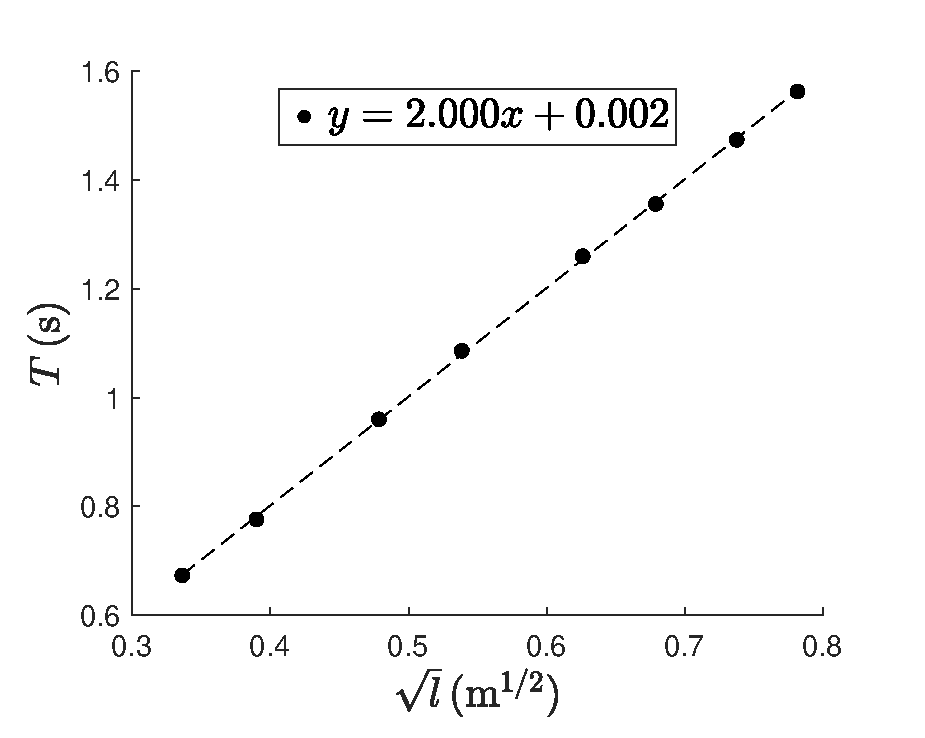
\includegraphics[width=0.8\columnwidth]{files/images/fig1}
    \end{center}
    \caption{Masa 1 - Periodo frente a ra�z cuadrada de la longitud.}
    \label{fig:r1}
\end{figure}

La pendiente de la gr�fica~\ref{fig:r1}, incluida su desviaci�n est�ndar como error, es:
\begin{equation*}
    \frac{2\pi}{\sqrt{g}} = (2,024 \pm 0.010)\, \text{s/m$^{1/2}$}
\end{equation*}

De esta ecuaci�n, despejamos $g$ y obtenemos:
\begin{equation*}
    g = (9,64 \pm 0.10)\, \text{m/s$^2$}
\end{equation*}

\begin{figure}[tbh]
    \begin{center}
        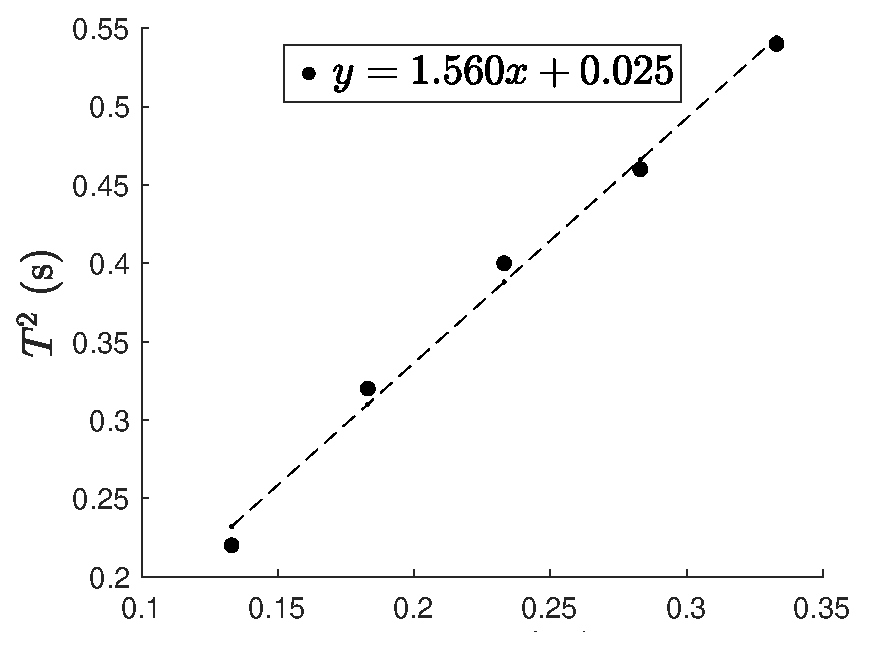
\includegraphics[width=0.8\columnwidth]{files/images/fig2}
    \end{center}
    \caption{Masa 1 - Periodo al cuadrado frente a longitud.}
    \label{fig:r2}
\end{figure}

La pendiente de la gr�fica~\ref{fig:r2} es:
\begin{equation*}
    \frac{g}{4\pi^2} =  (0.2467 \pm 0.0013)\, \text{m/s$^{2}$}
\end{equation*}

De ah�:
\begin{equation*}
    g = (9,74 \pm 0.05)\, \text{m/s$^2$}
\end{equation*}


\begin{figure}[tbh]
    \begin{center}
        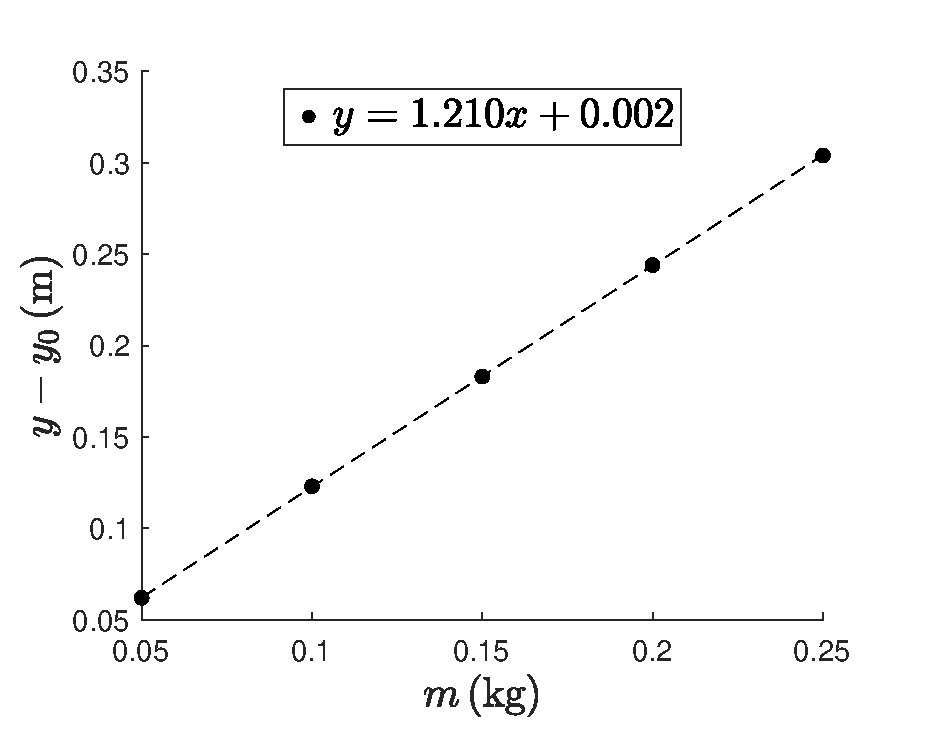
\includegraphics[width=0.8\columnwidth]{files/images/fig3}
    \end{center}
    \caption{Masa 1 - Periodo frente a longitud.}
    \label{fig:r3}
\end{figure}

Se agrupan en una l�nea de pendiente 2.


